% ****** Start of file apssamp.tex ******
%
%   This file is part of the APS files in the REVTeX 4.2 distribution.
%   Version 4.2a of REVTeX, December 2014
%
%   Copyright (c) 2014 The American Physical Society.
%
%   See the REVTeX 4 README file for restrictions and more information.
%
% TeX'ing this file requires that you have AMS-LaTeX 2.0 installed
% as well as the rest of the prerequisites for REVTeX 4.2
%
% See the REVTeX 4 README file
% It also requires running BibTeX. The commands are as follows:
%
%  1)  latex apssamp.tex
%  2)  bibtex apssamp
%  3)  latex apssamp.tex
%  4)  latex apssamp.tex
%
\documentclass[%
 reprint,
%superscriptaddress,
%groupedaddress,
%unsortedaddress,
%runinaddress,
%frontmatterverbose, 
%preprint,
%preprintnumbers,
%nofootinbib,
%nobibnotes,
%bibnotes,
 amsmath,amssymb,
 aps,
%pra,
%prb,
%rmp,
%prstab,
%prstper,
%floatfix,
]{revtex4-2}

\usepackage{graphicx}% Include figure files
\usepackage{dcolumn}% Align table columns on decimal point
\usepackage{bm}% bold math
\usepackage{subfigure}
\usepackage{lineno}
%\usepackage{hyperref}% add hypertext capabilities
%\usepackage[mathlines]{lineno}% Enable numbering of text and display math
%\linenumbers\relax % Commence numbering lines

%\usepackage[showframe,%Uncomment any one of the following lines to test 
%%scale=0.7, marginratio={1:1, 2:3}, ignoreall,% default settings
%%text={7in,10in},centering,
%%margin=1.5in,
%%total={6.5in,8.75in}, top=1.2in, left=0.9in, includefoot,
%%height=10in,a5paper,hmargin={3cm,0.8in},
%]{geometry}

\begin{document}

\preprint{}

\title{Joint WAGASCI+ND280 CC0 $\pi^{\pm}$ Cross-section Measurement on Water and Hydrocarbon Technical Note}

\collaboration{T2K Collaboration}%\noaffiliation

\author{J.~C.~Nugent}
\affiliation{
Tohoku University, Faculty of Science, Department of Physics, Miyagi, Japan
}

\date{\today}% It is always \today, today,
             %  but any date may be explicitly specified

\begin{abstract}
 
\end{abstract}

%\keywords{Suggested keywords}%Use showkeys class option if keyword
                              %display desired
\maketitle

%\tableofcontents

\section{\label{Sect:Intro}INTRODUCTION}

We report a cross-section measurement of $\nu_{\mu}$ on water and hydrocarbon interacting via a charged current quasi-elastic reaction using two T2K near detectors, WAGASCI and ND280. A leading source of uncertainty in the neutrino oscillation measurements is due to uncertainties in neutrino interaction models. Collecting new data on these two critical nuclear targets and exploiting the correlations at multiple off-axis angle to make cross-sections of greater sensitivity will address this issue and improve the sensitivity of future neutrino oscillation measurements. A two dimensional fit was made in the resultant lepton kinematics of momentum and angle with two one dimenisional results extracted due to the limited statistics in the WAGASCI sample. We report a total integrated measured cross-section of XX in muon momentum and a total integrated measured cross-section of YY in muon angle. The result was compared to model predictions provided by NEUT blahblah and GENIE blahblah and the measured result is/is not compatible these models.

\section{\label{Sect:Method}The T2K experiment}

The Tokai-2-Kamiokande (T2K) experiment \cite{} is a long-base line neutrino experiment located in Japan. The far detector is the SuperKamiokande detector \cite{} located 295 km from J-PARC which produces the $\nu$ beam at 2.5$^\circ$ off-axis which means a narrow band $\nu$ beam can be studied. This narrow band beam is peaked at 0.6\,GeV and contains less than 1\% $\nu_e$ contamination. Before the neutrino beam travels through the earth to the FD and oscillates it is measured at the near-detector complex which houses multiple detectors including WAGASCI and ND280. 
\begin{figure*}[htbp]
\begin{center}
\includegraphics[width=\textwidth]{_cooling_channel.pdf}
\end{center}
\caption{Schematic of the MICE cooling channel. The spectrometer solenoids and focus coils were not powered during the measurements described here. A variable thickness diffuser upstream of the trackers was fully retracted during the measurements. Acronyms are defined in the text.}
\label{fig:micecc}
\end{figure*}

\begin{table*}
\caption{Material budget affecting particles passing through the MICE LiH
  absorber. The material thickness normalized by the radiation length
  is given with the RMS width of the scattering distribution calculated from
  the full PDG formula \cite{Zyla:2020zbs} in eq. \ref{eq:pdg}. Note that the 
  thickness shown for the tracker materials (He, Al windows and Scintillating Fibres) includes 
  both trackers.}
\label{tab:RMSpred}
\vspace{3mm}
\centering
\begin{ruledtabular}
\begin{tabular}{c|ccc|ccc}
% {|c|ccc|ccc|}
%\hline
& & & & \multicolumn{3}{c}{$\theta_0$ (mrad)} \\ 
Material & $z$ (cm) & $z/X_{0}$ & $\rho$ (g cm$^{-3}$) & 172\,MeV/$c$ & 200\,MeV/$c$ & 240\, MeV/$c$ \\ 
\hline
Tracker He & 226 & 0.00030 & 1.663$\times$10$^{-4}$ & 1.09 & 0.91 & 0.73 \\ 
Al Window & 0.032 & 0.0036 & 2.699 & 4.31 & 3.58 & 2.89 \\ 
Scintillating Fibres & 1.48 & 0.036 & 1.06 & 14.9 & 12.4 & 10.0 \\
Total Tracker &  & 0.038 & & 15.8 & 13.2 & 10.6 \\
LiH & 6.5 &  0.0641 & 0.6957      & 21.3 & 17.7 & 14.3 \\ % & 0.001 \\
\hline
Total with LiH & & 0.1058 & & 29.9 & 24.8 & 20.0 \\
%\hline
\end{tabular}
\end{ruledtabular}
\end{table*}

\section{\label{Sect:Data}The muon neutrino beam}
\begin{figure*}[htbp]
\begin{center}
\includegraphics[width=\textwidth]{_cooling_channel.pdf}
\end{center}
\caption{Schematic of the MICE cooling channel. The spectrometer solenoids and focus coils were not powered during the measurements described here. A variable thickness diffuser upstream of the trackers was fully retracted during the measurements. Acronyms are defined in the text.}
\label{fig:micecc}
\end{figure*}

The J-PARC accelerator produces 30\,GeV protons that are incident on a graphite target. The resultant interaction produces pions which are focused in the direction of the T2K detectors by 3 magnetic horns. The magnetic horns also defocus pions with the wrong signed charge ensuring greater purity of the neutrino vs. nti neutrino content of the resultant beam. The beam then enters the decay pipe and over the next 80 meters pions decay producing a tertiary beam of neutrinos travelling in the direction of Kamioka. 

\subsection{The T2K near detectors}
\begin{figure*}[htbp]
\begin{center}
\includegraphics[width=\textwidth]{_cooling_channel.pdf}
\end{center}
\caption{Schematic of the MICE cooling channel. The spectrometer solenoids and focus coils were not powered during the measurements described here. A variable thickness diffuser upstream of the trackers was fully retracted during the measurements. Acronyms are defined in the text.}
\label{fig:micecc}
\end{figure*}
\begin{figure*}[htbp]
\begin{center}
\includegraphics[width=\textwidth]{_cooling_channel.pdf}
\end{center}
\caption{Schematic of the MICE cooling channel. The spectrometer solenoids and focus coils were not powered during the measurements described here. A variable thickness diffuser upstream of the trackers was fully retracted during the measurements. Acronyms are defined in the text.}
\label{fig:micecc}
\end{figure*}

280\,m from the target station the T2K near detectors measure the neutrino flux before the neutrinos leave J-PARC and oscillate. ND280 is a tracking detector composed of FGDs 1 \& 2 (Fine-Grained Detectors), made of scintillator bars, and TPCs (Time Projection Chambers), filled with gas which can measure particle momentum and $dE/dx$ for particle identification (PID). The entire ND280 is encased in the Ecal and electromagnetic calorimeter used for measuring energt deposition. 

WAGASCI is the newest T2K ND with installation having been completed in 2020. The main WAGASCI modules are water tanks filled with grid and planes of scintillator. This presents two critical nuclear interaction targets, water and hydrocarbon, with the scintillator readout being used for event reconstruction. 
\subsection{Sample definition}
\label{sec:selection}

\subsection{Signal definition}
\label{sec:seldef}
\begin{figure*}[htbp]
\begin{center}
\includegraphics[width=\textwidth]{_cooling_channel.pdf}
\end{center}
\caption{Schematic of the MICE cooling channel. The spectrometer solenoids and focus coils were not powered during the measurements described here. A variable thickness diffuser upstream of the trackers was fully retracted during the measurements. Acronyms are defined in the text.}
\label{fig:micecc}
\end{figure*}
\begin{figure*}[htbp]
\begin{center}
\includegraphics[width=\textwidth]{_cooling_channel.pdf}
\end{center}
\caption{Schematic of the MICE cooling channel. The spectrometer solenoids and focus coils were not powered during the measurements described here. A variable thickness diffuser upstream of the trackers was fully retracted during the measurements. Acronyms are defined in the text.}
\label{fig:micecc}
\end{figure*}
\begin{figure*}[htbp]
\begin{center}
\includegraphics[width=\textwidth]{_cooling_channel.pdf}
\end{center}
\caption{Schematic of the MICE cooling channel. The spectrometer solenoids and focus coils were not powered during the measurements described here. A variable thickness diffuser upstream of the trackers was fully retracted during the measurements. Acronyms are defined in the text.}
\label{fig:micecc}
\end{figure*}

The signal for this analysis is CC0$\pi$, so a charged current interaction which results in no measured pions in the FS. To allow for freedom when comparing to models multiple tracks are allowed provided that they are indentified as muon like. The resultant $mu$ from the neutrino interaction in WAGASCI topologies listed here 
\begin{itemize}
    \item a WAGASCI module to a WMRD or BabyMIND
    \item the proton module to a WRMD or BabyMIND
\end{itemize} 
will be used. In the case of ND280 any topologies listed here:
\begin{itemize}
    \item $\mu$TPC 
    \item $\mu$TPC+pTPC
    \item $\mu$TPC+pFGD
    \item $\mu$TPC+Np
    \item $\mu$FGD 
    \item $\mu$FGD+pTPC 
\end{itemize} 
will be used. 

\subsection{Sideband definition}
\label{sec:sideband}

Sidebands for WAGASCI are events which match the CC1$\pi$ topoogy definition. So any interaction which includes 1 pion in the FS. For ND280 the sidebands are defined as CC1$\pi$ events (any event with 1 pion in the FS) or DIS (events which liberate multiple pions which are detected in the FS).

\subsection{Signal and background selection}
\label{sec:selection}

Events for this analysis will be selected based on the schemes described in TN455 \ref{} for WAGASCI and TNYY \ref{} for ND280. The primary purpose of this analysis is to harmonise the analyses of these two diferent detectors, as such, further improving the efficiencies or purities of the previously defined selections was not a priority. Significant effort was made to ensure consistenancy is the MC generation and analysis framework, including switching from a standalone framework for WAGASCI to Highland2, the framework most commonly used throughout T2K and by ND280 for event selection and Detector Systematics. 

As such, while plots will be presented in this section detailing each cut parameter and muon kinematics for WAGASCI no changes have been made to the selection scheme from TN455. The goal is for all plots to be consistent with those reported in the previous TN but with the new MC and produced in the new analysis framework. This will ensure that no unintended changes have been introduced the migration. While the previous selection has already been approved and hence the selection should in principle be able to be used without incident, nevertheless, all plots will be reviewed afresh to ensure that they are suitable for this new joint analysis. 

As the ND280 selection scheme has not changed and there has been no migration of software or significant changes to the MC, this selection should be usable without issue. All kinematic plots will be included here for completeness and checked for consistency in this analysis but as the event selection has been stable for some time and no modifications are being made in this analysis these plots should, in principle, only be for information. 

For full details of the selection scheme and a description of the cuts used for each detector please consult the relevant TN cited above.

\subsection{WAGASCI event selection}
\begin{figure*}[htbp]
\begin{center}
\includegraphics[width=\textwidth]{_cooling_channel.pdf}
\end{center}
\caption{Schematic of the MICE cooling channel. The spectrometer solenoids and focus coils were not powered during the measurements described here. A variable thickness diffuser upstream of the trackers was fully retracted during the measurements. Acronyms are defined in the text.}
\label{fig:micecc}
\end{figure*}
    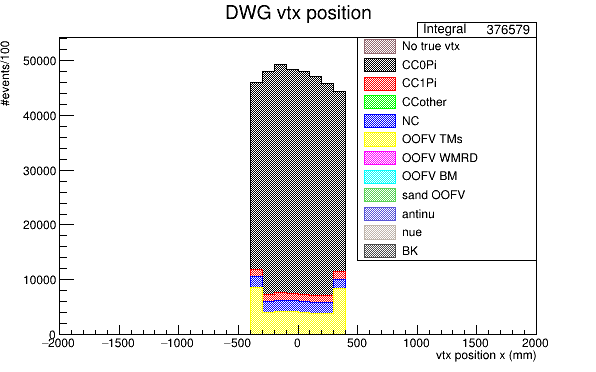
\includegraphics[width=0.45\textwidth]{images/vtx_reco_pos[0]_wgbm_topo_DWG_accum_level[][26]_data_mc.png}
    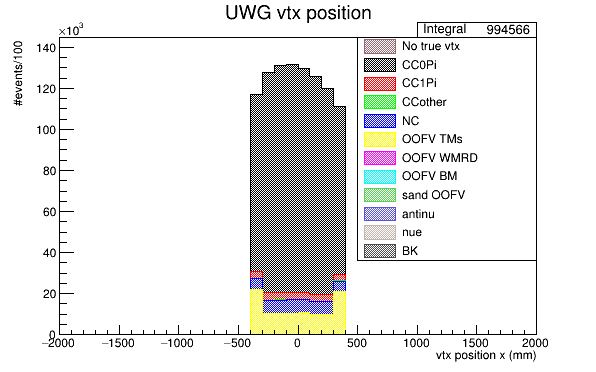
\includegraphics[width=0.45\textwidth]{images/vtx_reco_pos[0]_wgbm_topo_UWG_accum_level[][16]_data_mc.png}
    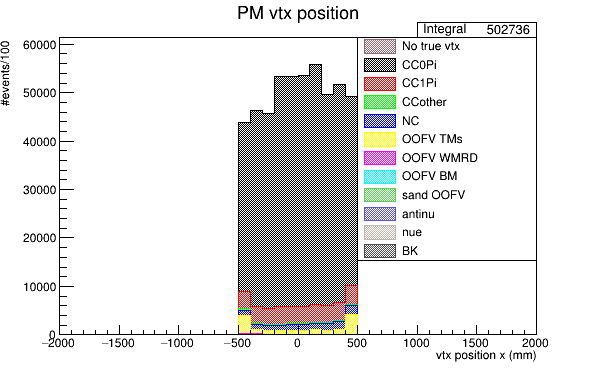
\includegraphics[width=0.45\textwidth]{images/vtx_reco_pos[0]_wgbm_topo_PM_accum_level[][06]_data_mc.png}
\end{frame}

\begin{frame}{Vertex}
    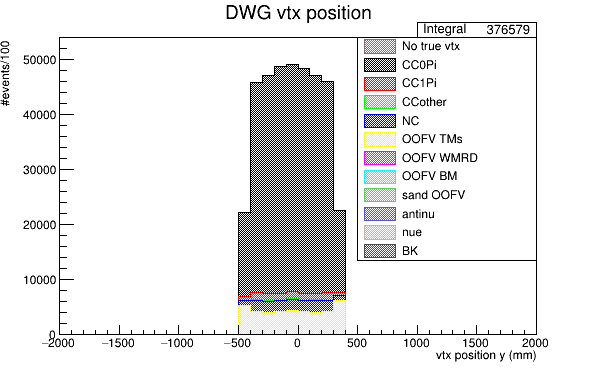
\includegraphics[width=0.45\textwidth]{images/vtx_reco_pos[1]_wgbm_topo_DWG_accum_level[][26]_data_mc.png}
    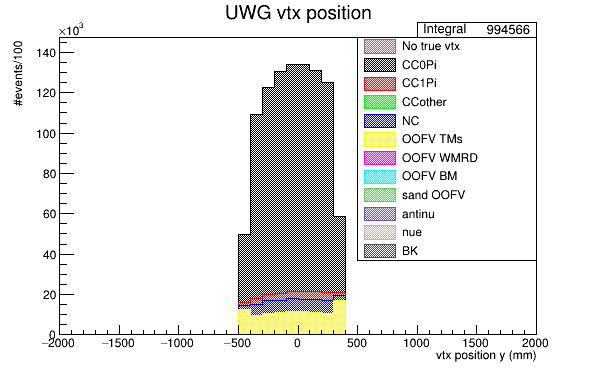
\includegraphics[width=0.45\textwidth]{images/vtx_reco_pos[1]_wgbm_topo_UWG_accum_level[][16]_data_mc.png}
    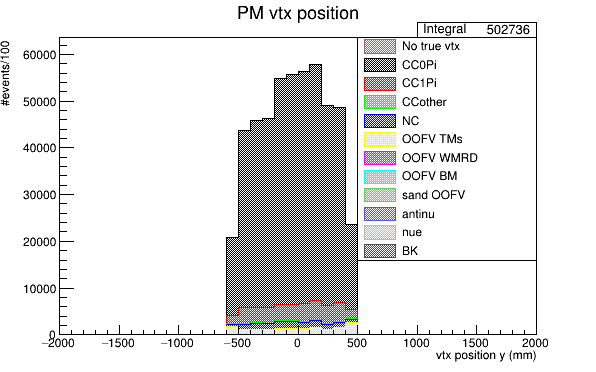
\includegraphics[width=0.45\textwidth]{images/vtx_reco_pos[1]_wgbm_topo_PM_accum_level[][06]_data_mc.png}
    \end{frame}

\begin{frame}{Vertex}
    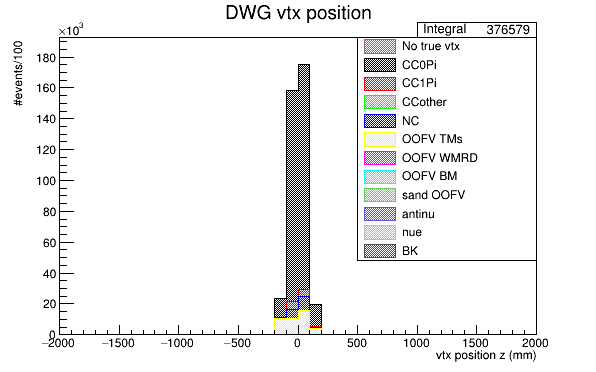
\includegraphics[width=0.45\textwidth]{images/vtx_reco_pos[2]_wgbm_topo_DWG_accum_level[][26]_data_mc.png}
    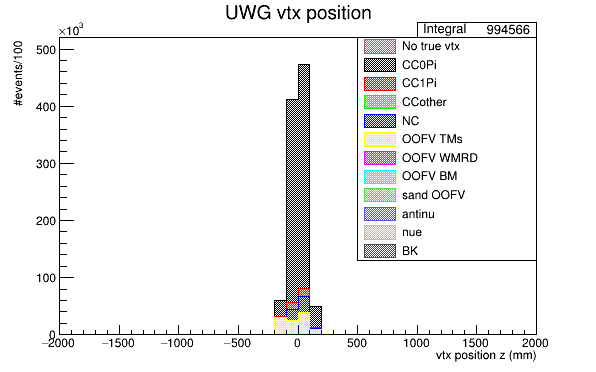
\includegraphics[width=0.45\textwidth]{images/vtx_reco_pos[2]_wgbm_topo_UWG_accum_level[][16]_data_mc.png}
    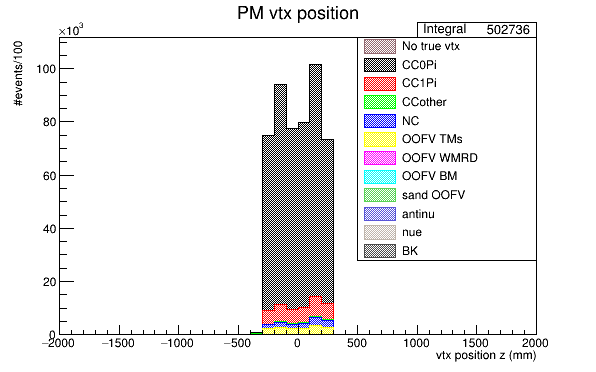
\includegraphics[width=0.45\textwidth]{images/vtx_reco_pos[2]_wgbm_topo_PM_accum_level[][06]_data_mc.png}
\end{frame}

\begin{frame}{No. of tracks}
    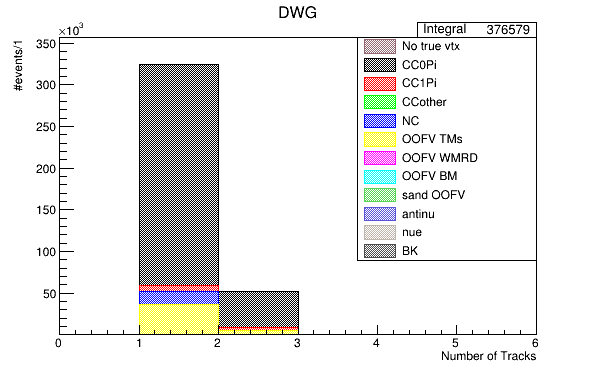
\includegraphics[width=0.45\textwidth]{images/num_of_vtx_reco_tracks_wgbm_topo_DWG_accum_level[][26]_data_mc.png}
    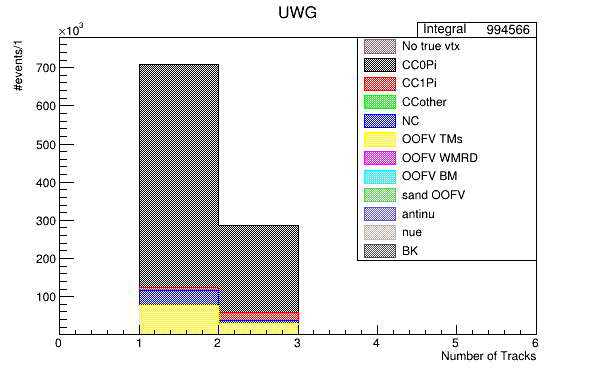
\includegraphics[width=0.45\textwidth]{images/num_of_vtx_reco_tracks_wgbm_topo_UWG_accum_level[][16]_data_mc.png}
    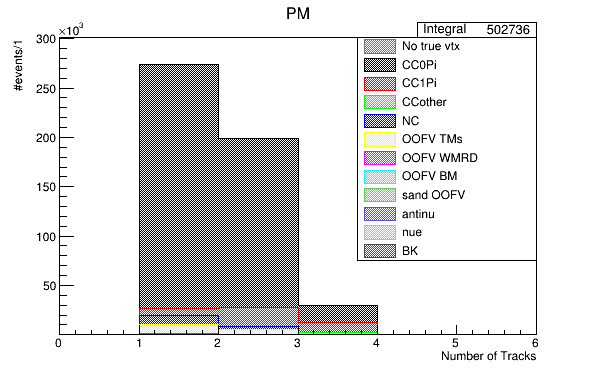
\includegraphics[width=0.45\textwidth]{images/num_of_vtx_reco_tracks_wgbm_topo_PM_accum_level[][06]_data_mc.png}
\end{frame}

\begin{frame}{$\mu$ CL}
    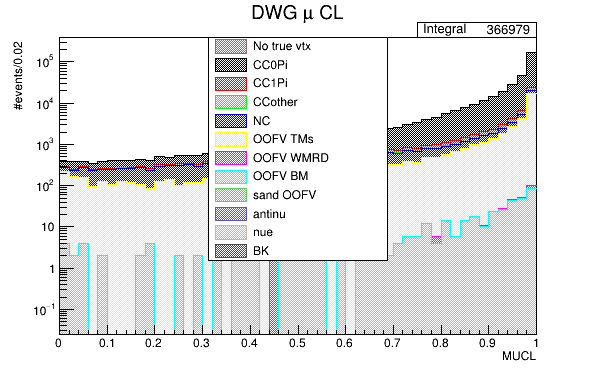
\includegraphics[width=0.45\textwidth]{images/mucl_dwg_wgbm_topo_DWG_accum_level[][26]_data_mc.png}
    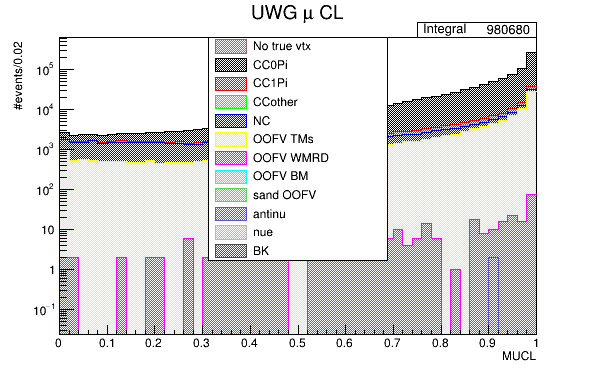
\includegraphics[width=0.45\textwidth]{images/mucl_uwg_wgbm_topo_UWG_accum_level[][16]_data_mc.png}
    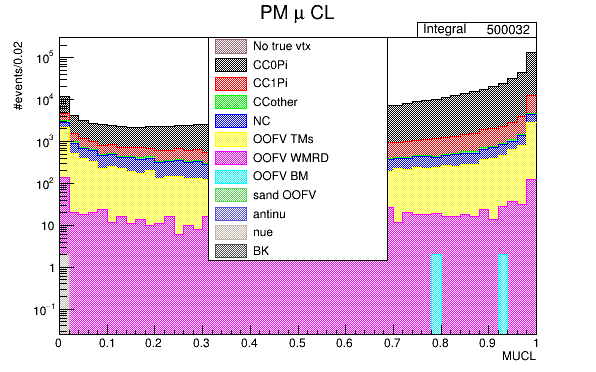
\includegraphics[width=0.45\textwidth]{images/mucl_pm_wgbm_topo_PM_accum_level[][06]_data_mc.png}
    \end{frame}

\begin{frame}{Charge -ve}
    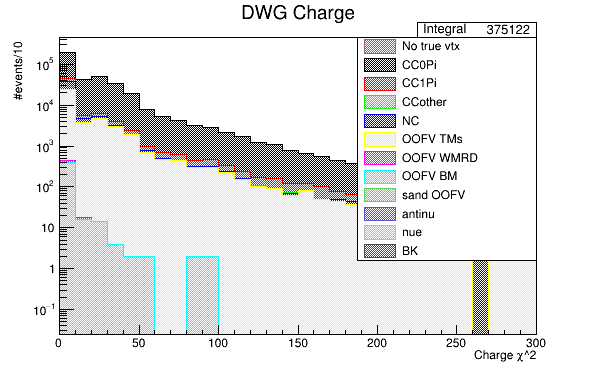
\includegraphics[width=0.45\textwidth]{images/charge_neg_chi2_wgbm_topo_DWG_accum_level[][26]_data_mc.png}
    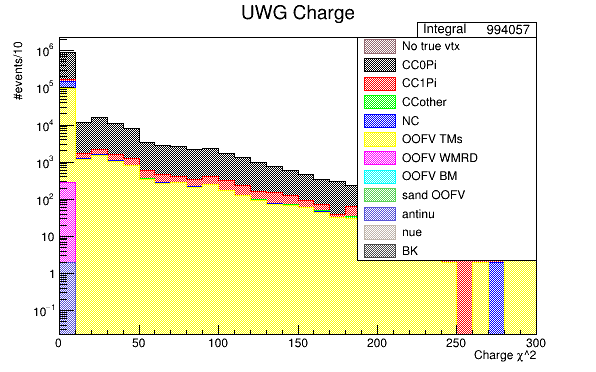
\includegraphics[width=0.45\textwidth]{images/charge_neg_chi2_wgbm_topo_UWG_accum_level[][16]_data_mc.png}
    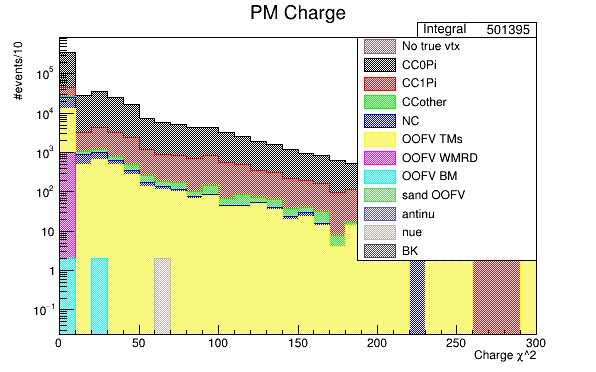
\includegraphics[width=0.45\textwidth]{images/charge_neg_chi2_wgbm_topo_PM_accum_level[][06]_data_mc.png}
\end{frame}

\begin{frame}{Charge +ve}
    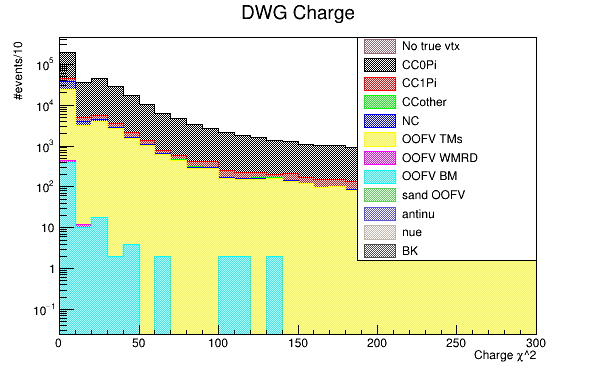
\includegraphics[width=0.45\textwidth]{images/charge_pos_chi2_wgbm_topo_DWG_accum_level[][26]_data_mc.png}
    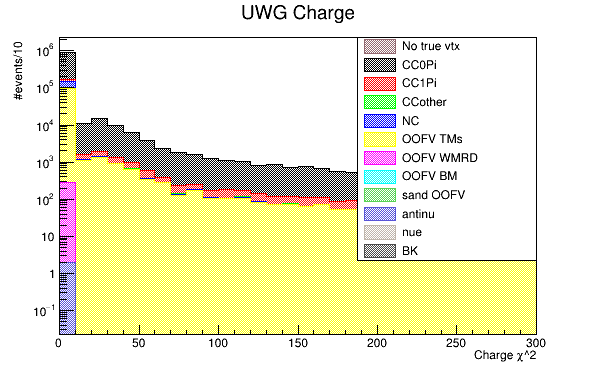
\includegraphics[width=0.45\textwidth]{images/charge_pos_chi2_wgbm_topo_UWG_accum_level[][16]_data_mc.png}
    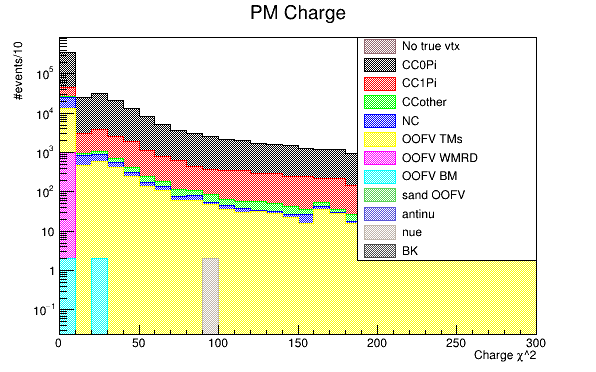
\includegraphics[width=0.45\textwidth]{images/charge_pos_chi2_wgbm_topo_PM_accum_level[][06]_data_mc.png}
\end{frame}

\begin{frame}{Track to cluster ratio}
    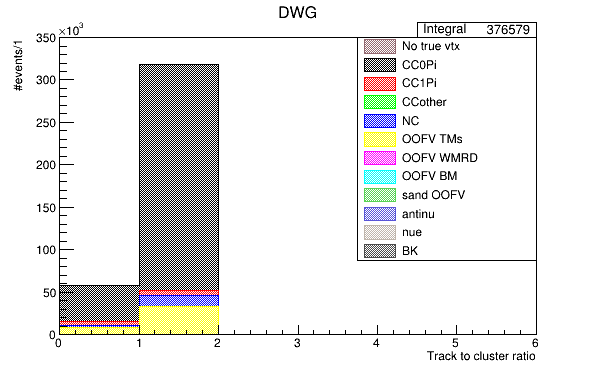
\includegraphics[width=0.45\textwidth]{images/track_to_cluster_hits_ratio_wgbm_topo_DWG_accum_level[][26]_data_mc.png}
    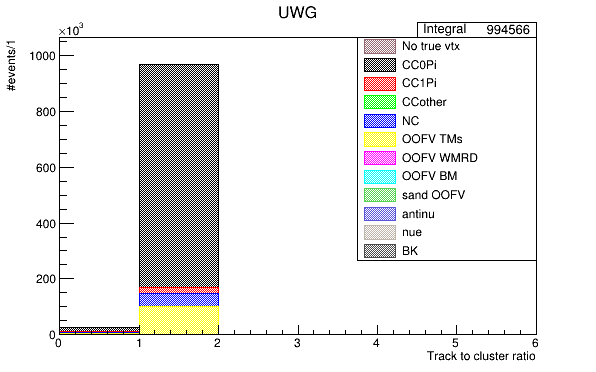
\includegraphics[width=0.45\textwidth]{images/track_to_cluster_hits_ratio_wgbm_topo_UWG_accum_level[][16]_data_mc.png}
    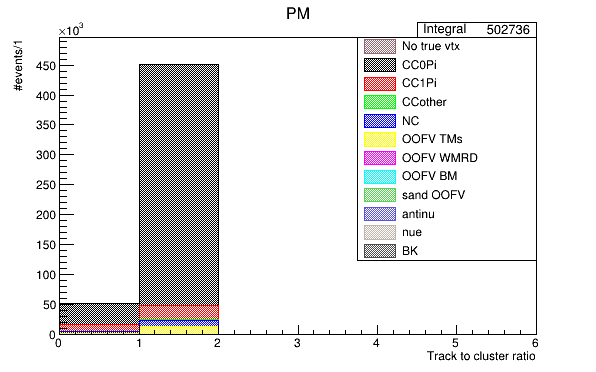
\includegraphics[width=0.45\textwidth]{images/track_to_cluster_hits_ratio_wgbm_topo_PM_accum_level[][06]_data_mc.png}
\end{frame}

\begin{frame}{No. of delayed hits}
    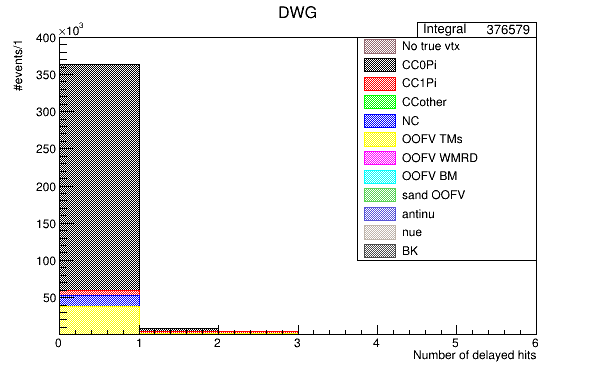
\includegraphics[width=0.45\textwidth]{images/num_reco_delayed_hits_wgbm_topo_DWG_accum_level[][26]_data_mc.png}
    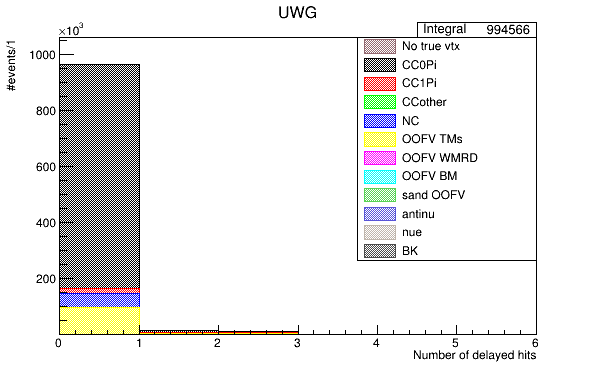
\includegraphics[width=0.45\textwidth]{images/num_reco_delayed_hits_wgbm_topo_UWG_accum_level[][16]_data_mc.png}
    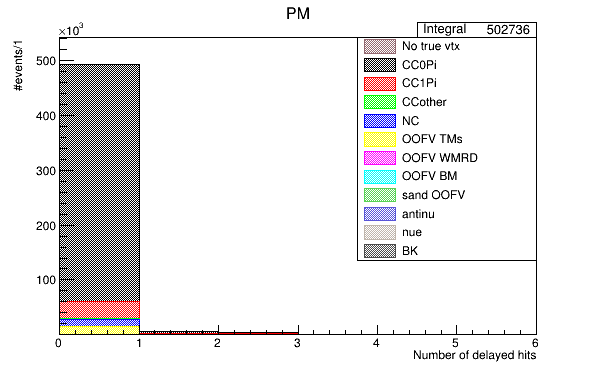
\includegraphics[width=0.45\textwidth]{images/num_reco_delayed_hits_wgbm_topo_PM_accum_level[][06]_data_mc.png}
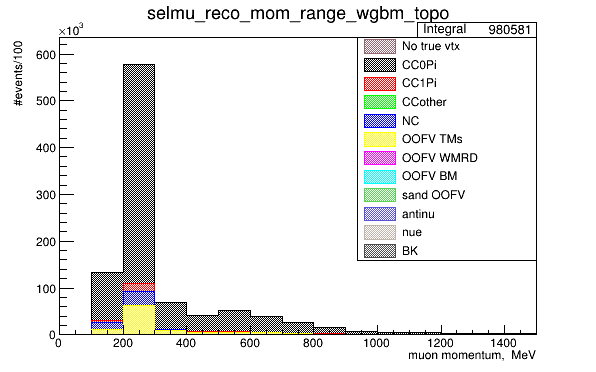
\includegraphics[width=.45\textwidth]{images/selmu_reco_mom_range_UWG_wgbm_topo_accum_level[][16]_data_mc.png}
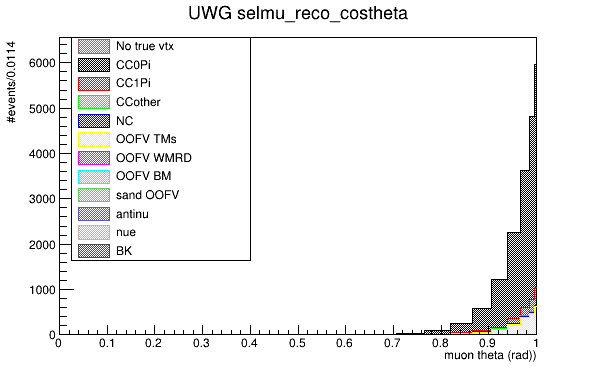
\includegraphics[width=.45\textwidth]{images/selmu_reco_costheta_wgbm_topo_UWG_accum_level[][16]_data_mc.png}
\end{frame}
\begin{frame}{UWG}
\center
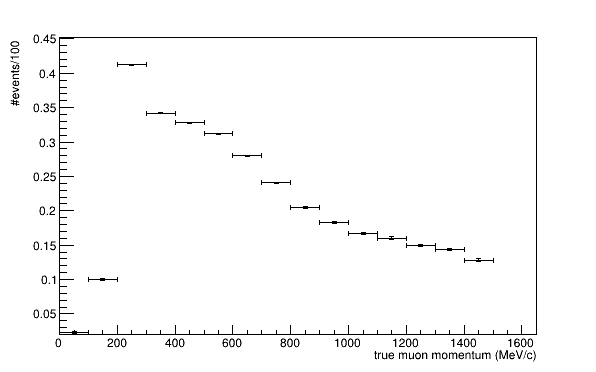
\includegraphics[width=.45\textwidth]{images/Eff_selmu_true_mom_wgbm_topo_UWG_accum_level[][16]_data_mc.png}
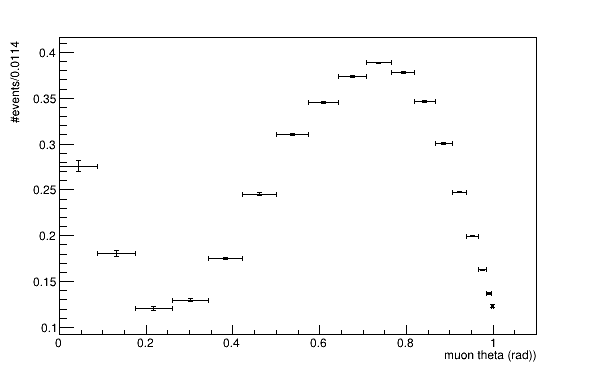
\includegraphics[width=.45\textwidth]{images/Eff_selmu_true_costheta_wgbm_topo_UWG_accum_level[][16]_data_mc.png}
\end{frame}
\begin{frame}{UWG}
\center
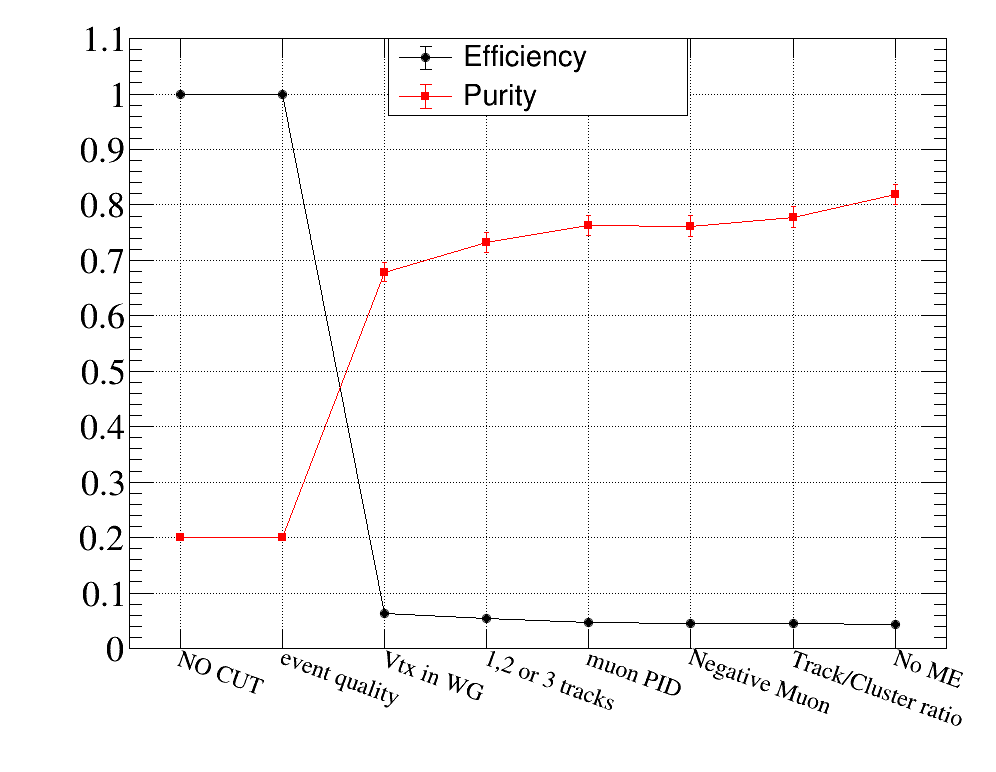
\includegraphics[width=.45\textwidth]{images/EffPurVsCut_br1_true_wgbm_topo.png}
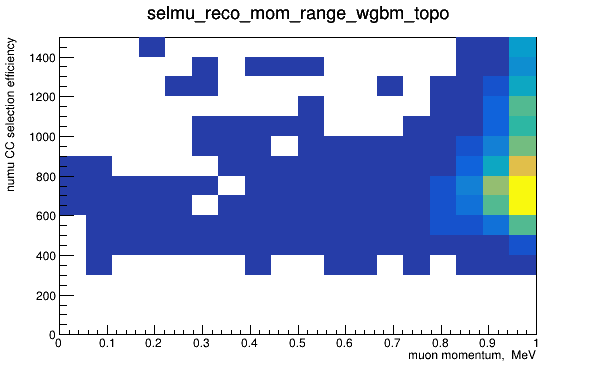
\includegraphics[width=.45\textwidth]{images/2D_selmu_mom:selmu_costheta_wgbm_topo_accum_level[][16]_data_mc.png}
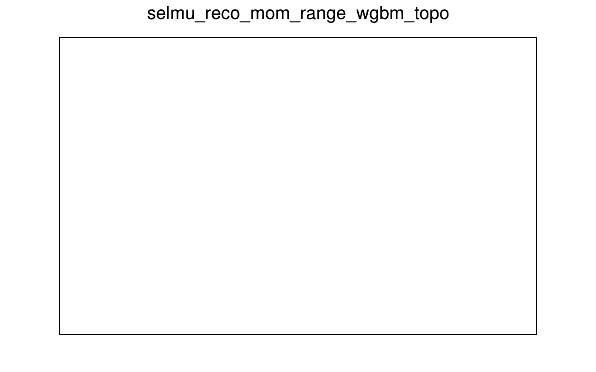
\includegraphics[width=.45\textwidth]{images/ratio_selmu_reco_mom_range_wgbm_topo_accum_level[][16]_data_mc.png}
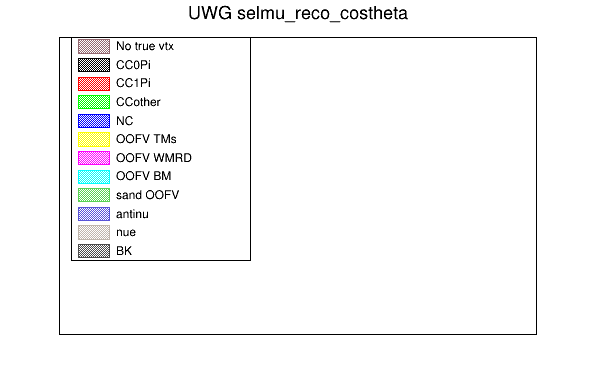
\includegraphics[width=.45\textwidth]{images/ratio_selmu_reco_costheta_wgbm_topo_UWG_accum_level[][16]_data_mc.png}
 
 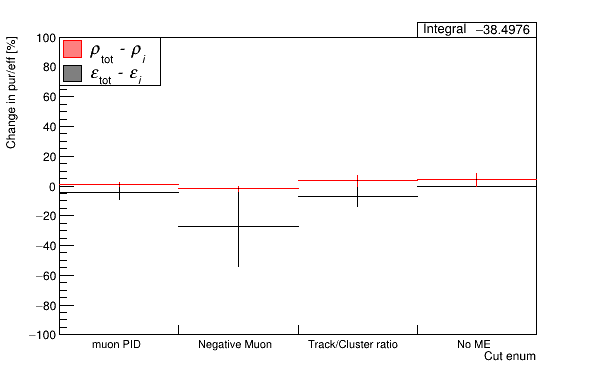
\includegraphics[width=.45\textwidth]{images/nMinusOneCuts_sample2.png}
    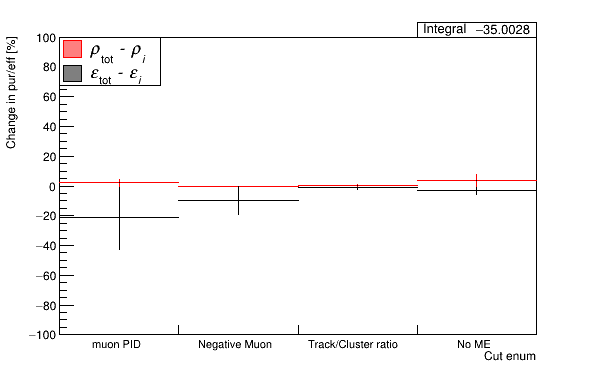
\includegraphics[width=.45\textwidth]{images/nMinusOneCuts_sample1.png}
    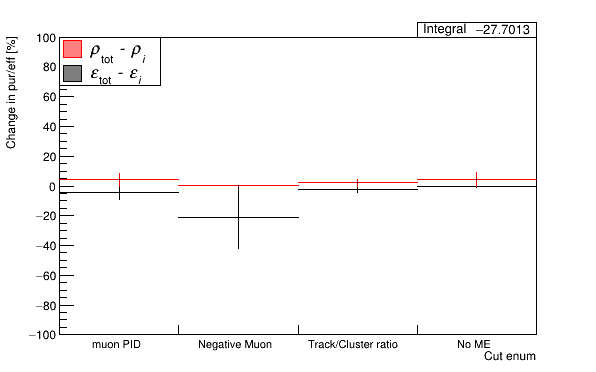
\includegraphics[width=.45\textwidth]{images/nMinusOneCuts_sample0.png}
\subsection{ND280 event selection}
\begin{figure*}[htbp]
\begin{center}
\includegraphics[width=\textwidth]{_cooling_channel.pdf}
\end{center}
\caption{Schematic of the MICE cooling channel. The spectrometer solenoids and focus coils were not powered during the measurements described here. A variable thickness diffuser upstream of the trackers was fully retracted during the measurements. Acronyms are defined in the text.}
\label{fig:micecc}
\end{figure*}

\subsection{Detector Systematics}
\label{sec:selection}

\subsection{Fake data studies}

\subsection{Results}

\section{\label{Sect:Results}Conclusion}

\section{\label{Sect:Conclusions}CONCLUSIONS}

Presented here is an analysis of the $\nu_{\mu}$ cross-section of water and hydrocarbon in the WAGASCI and ND280 detectors using XX POT of data collected during J-PARC Run 10 and 11 (XX/YY/ZZZ). These data were compared to the GENIE (vX.X) \cite{} and the NEUT prediction \cite{}. In the lepton kinematics reported in the measurement the data and model show good/bad/terrible compatibility. 
\newpage
\appendix*

\section{\label{Sect:Appendix}Definition of Scattering Angles}


\begin{acknowledgments}
The work described here was made possible by grants from the Science and Technology Facilities Council (UK), the Department of Energy and the National Science Foundation (USA), the Istituto Nazionale di Fisica Nucleare (Italy), the European Union under the European Union’s Framework Programme 7 (AIDA project, grant agreement number 262025; TIARA project, grant agreement number 261905; and EuCARD), the Japan Society for the Promotion of Science, the National Research Foundation of Korea (number NRF-2016R1A5A1013277), the Ministry of Education, Science and Technological Development of the Republic of Serbia, the Institute of High Energy Physics/Chinese Academy of Sciences fund for collaboration between the People’s Republic of China and the USA, and the Swiss National Science Foundation in the framework of the SCOPES programme. We gratefully acknowledge all sources of support. We are grateful for the support given to us by the staff of the STFC Rutherford Appleton and Daresbury laboratories. We acknowledge the use of Grid computing resources deployed and operated by GridPP in the UK, http://www.gridpp.ac.uk/.

\end{acknowledgments}

We thank the J-PARC staff for superb accelerator performance. We thank the CERN NA61/SHINE Collaboration for providing valuable particle production data. We acknowledge the support of MEXT, JSPS KAKENHI Grants No. JP16H06288, No. JP18K03682,
No. JP18H03701, No. JP18H05537, No. JP19J01119, No. JP19J22440, No. JP19J22258, No. JP20H00162, No. JP20H00149, and No. JP20J20304) and bilateral programs (JPJSBP120204806, JPJSBP120209601), Japan; NSERC, the NRC, and CFI, Canada; the CEA and
CNRS/IN2P3, France; the DFG (RO 3625/2), Germany; the INFN, Italy; the Ministry of Education and Science (DIR/WK/2017/05) and the National Science Centre (UMO-2018/30/E/ST2/00441), Poland; the RSF19-12-00325, RSF22-12-00358, Russia; MICINN (No. SEV-2016-0588, No. PID2019–107564 GB-I00, No. PGC2018-099388-BI00, No. PID2020–114687 GB-I00) Government of Andalucia (FQM160, SOMM17/6105/UGR) and the University of Tokyo ICRR’s Inter-University Research Program FY2023 Ref. J1, and ERDF funds and CERCA program, Spain; the SNSF and SERI(200021\_185012, 200020\_188533, 20FL21\_186178I), Switzerland; the STFC and UKRI, UK; and the DOE, USA. We also thank CERN for the UA1/NOMAD magnet, DESY for the HERA-B magnet mover system, the BC DRI Group, Prairie DRI Group, ACENET, SciNet, and CalculQuebec consortia in the Digital Research Alliance of Canada, and GridPP in the United Kingdom, and the CNRS/IN2P3 Computing Center in France. In addition, the participation of individual researchers and institutions has been further supported by funds from the ERC (FP7), “la Caixa” Foundation (ID 100010434, Fellowship Code No. LCF/BQ/IN17/11620050), the European Union’s Horizon 2020 Research and Innovation Programme under
the Marie Sklodowska-Curie Grants Agreement No. 713673  and No. 754496, and H2020 Grants No. RISE-GA822070-JENNIFER2 2020 and No. RISE-GA872549-SK2HK; the JSPS, Japan; the Royal Society, UK; French ANR Grant No. ANR-19-CE31-0001; the SNF Eccellenza Grant No. PCEFP2\_203261; and the DOE Early Career program, USA.
\appendix

\bibliography{apssamp}% Produces the bibliography via BibTeX.

%\input AuthorList
\end{document}
%
% ****** End of file apssamp.tex ******
